\documentclass{article}
\usepackage[utf8]{inputenc}
\usepackage[T1]{fontenc}
\usepackage[french]{babel}
\usepackage{amsmath, amssymb, amsthm}
\usepackage{geometry}
\usepackage{titling}
\usepackage{fancyhdr}
\usepackage{lipsum}
\usepackage{parskip}
\usepackage{forest}
\usepackage{tikz}
\usepackage{stmaryrd}
\usepackage{listings}
\usepackage{graphicx}
\usepackage{float}

\geometry{top=4cm, bottom=4cm, left=4cm, right=4cm}
\pagestyle{fancy}
\fancyhf{}
\rhead{Pierre Pili}
\lhead{International Macroeconomics - Homework 1}
\cfoot{\thepage}

\title{INTERNATIONAL MACRO - HOMEWORK 1}
\author{Pierre Pili}
\date{\today}

\begin{document}

\begin{titlingpage}
\maketitle
\end{titlingpage}

\tableofcontents

\newpage
\section{A 3-Period Model}
\subsection{}
One can derive the following budget constraints from a 3-period small open endowment economy :
\begin{alignat}{2}
    C_1 + B_1 - B_0 &= Y_1 + r_0 B_0  \quad&\\
    C_2 + B_2 - B_1 &= Y_2 + r^* B_1  \quad&\\
    C_3 + B_3 - B_2 &= Y_3 + r^* B_2  \quad&
  \end{alignat}
Where $B_t$ and $Y_t$ are respectively the asset position and the endowment of households at period $t$.
\subsection{}
In a 3-period model, agents will not accumulate bonds in period three as they will not make it to the next period. They will rather maximize their consumption. Which implies $B_3 = 0$
\subsection{}
Rewriting (3) with the transversality condition :
\begin{alignat}{2}
    B_2 &= \frac{C_3 - Y_3}{1+r^*}  \quad&
\end{alignat}
Inserting the expression of $B_2$ in (2) :
\begin{alignat}{2}
    C_2 + \frac{C_3 - Y_3}{1+r^*} &= Y_2 + (1+r^*)B_1  \quad&
\end{alignat}
Which implies the following expression for $B_1$ :
\begin{alignat}{2}
    B_1 &= \frac{C_2 - Y_2}{1+r^*} + \frac{C_3 - Y_3}{(1+r^*)^2}  \quad&
\end{alignat}
Inserting the expression of $B_1$ in (1) :
\begin{alignat}{2}
    C_1 + \frac{C_2 - Y_2}{1+r^*} + \frac{C_3 - Y_3}{(1+r^*)^2} &= Y_1 + (1+r_0)B_0  \quad&
\end{alignat}
Rearranging (7) :
\begin{alignat}{2}
    C_1 + \frac{C_2}{1+r^*} + \frac{C_3}{(1+r^*)^2} &= (1+r_0)B_0 + Y_1 + \frac{Y_2}{1+r^*} + \frac{Y_3}{(1+r^*)^2} \equiv W \quad&
\end{alignat}
Where $W$ denotes the intertemporal wealth of households. $W$ is exogenous in this model since $Y_t, r_0, r^*$ and $B_0$ are exogenous.
\subsection{}
Households want to maximize their lifetime utiliy subject to the IBC. We thus form the lagrangian of this maximization problem :
\begin{alignat}{2}
    \mathcal{L}(C,\lambda) &= U(C) + \lambda \left[ W - \sum_t \frac{C_t}{(1+r^*)^{t-1}} \right] \quad&
\end{alignat}
Where $C$ is the vector of consumption $(C_1, C_2, C_3)$, $U$ the lifetime utility function, and where $\displaystyle\sum_t$ denotes the sum over all periods.\newline
The first order conditions imply, for $t \in$ $\{ 1, 2, 3\}$ :
\begin{alignat*}{2}
    \frac{\partial\mathcal{L}}{\partial C_t} (C,\lambda) = 0 &\iff C_t = \frac{(1+r^*)^{t-1}}{\lambda} \quad&
\end{alignat*}
Inserting the expressions for $C_t$ in the IBC implies :
\begin{alignat}{2}
    W = \sum_t \frac{1}{\lambda} &\iff \lambda = \frac{3}{W}\quad&
\end{alignat}
Which yields for $t \in$ $\{ 1, 2, 3\}$ :
\begin{alignat}{2}
    C_t &= \frac{(1+r^*)^{t-1}}{3}W\quad&
\end{alignat}
This result is similar to the 2-period economy with no discount factor for consumption in the lifetime utility.\newline
We can now easily compute the trade balance and the current account for each period :
\begin{alignat*}{2}
    TB_t &= Y_t - C_t\quad&\\
    &= Y_t - \frac{(1+r^*)^{t-1}}{3} \left[ (1+r_0)B_0 + Y_1 + \frac{Y_2}{1+r^*} + \frac{Y_3}{(1+r^*)^2} \right]\quad&\\
    &= \frac{(1+r^*)^{t-1}}{3} \left[\frac{3}{(1+r^*)^{t-1}}Y_t - (1+r_0)B_0 - Y_1 - \frac{Y_2}{1+r^*} - \frac{Y_3}{(1+r^*)^2} \right]\quad&
\end{alignat*}
Thus :
\begin{alignat}{2}
    TB_1 &= \frac{1}{3} \left[2 Y_1 -(1+r_0)B_0 - \frac{Y_2}{1+r^*} - \frac{Y_3}{(1+r^*)^2} \right]\quad&\quad&\\
    TB_2 &= \frac{(1+r^*)}{3} \left[\frac{2Y_2}{1+r^*} - (1+r_0)B_0 - Y_1 - \frac{Y_3}{(1+r^*)^2} \right]\quad&\\
    TB_3 &= \frac{(1+r^*)^2}{3} \left[\frac{2Y_3}{(1+r^*)^2} - (1+r_0)B_0 - Y_1 - \frac{Y_2}{(1+r^*)} \right]\quad&
\end{alignat}
\subsection{}
A positive endowment shock $\Delta Y_1$ will have a postive impact on the trade balance and on consumption in period 1, indeed, derivating (12) :
\begin{alignat}{2}
    \Delta TB_1 &= \Delta CA_1 = \frac{2}{3} \Delta Y_1  > 0 \quad&
\end{alignat}
Which implies,
\begin{alignat}{2}
    \Delta C_1 &= \frac{1}{3} \Delta Y_1  > 0 \quad&
\end{alignat}
\subsection{}
In a similar way, derivating (12) :
\begin{alignat}{2}
    \Delta TB_1 &= \Delta CA_1 = \Delta Y \left[2 - \frac{1}{1+r^*} - \frac{1}{(1+r^*)^2} \right] = \Delta Y \left[3 r^* + o(r^*)\right]\quad&
\end{alignat}
The trade balance in positively impacted by a permanent endowment shock but proportionnaly to $r^*$ at the first order. The impact will be very small.\newline
Thus permanent and transitory schocks have very different impact on the current account. While the former have a positive impact on the current account, the latter has almost no impact on it whatsoever. 
\begin{alignat*}{2}
    \Delta C_1 &= \Delta Y - \Delta TB_1 \quad&\\
    &= \Delta Y \left[1 - 3 r^* + o(r^*)\right]\quad&\\
\end{alignat*}
A permanent shock will increase consumption by a one-one coefficient at the first order with respect to $r^*$. 
\subsection{}
The way results were written so far very much suggests the general form of consumption in a N-period economy. The transversality condition writes $B_N = 0$.
In that case the intertemporal IBC writes :
\begin{alignat}{2}
    \sum_{t} \frac{C_t}{(1+r^*)^{(t-1)}} &= (1+r_0)B_0 + \sum_t \frac{Y_t}{(1+r^*)^{(t-1)}} \equiv W \quad&
\end{alignat}
The lagrangian is the same as in (9), which implies for any $t$ in $\llbracket 1, N \rrbracket$  that :
\begin{equation}{}
    C_t = \frac{(1+r^*)^{t-1}}{N}W 
\end{equation}
\begin{equation}{}
    TB_t = Y_t - \frac{(1+r^*)^{t-1}}{N} \left[ (1+r_0)B_0 - \sum_i \frac{Y_i}{(1+r^*)^{i-1}} \right]
    \label{tb_t}
\end{equation}
One is now able to redo question 1.5 and 1.6.\newline
\subsubsection*{1.5 bis}
Deriving \eqref{tb_t} for a positive endowment shock $\Delta Y_1$:
\begin{alignat*}{2}
    \Delta CA_1 = \Delta TB_1 &= \Delta Y_1 - \frac{1}{N} \Delta Y_1 \quad&\\
    &= \left[ 1 - \frac{1}{N}\right] \Delta Y_1 > 0 \quad&
    \label{Delta_tb}
\end{alignat*}
The trade balance in period 1 is positively impacted by a positive endowment shock in period 1. The variation in consumption writes :
\begin{alignat*}{2}
    \Delta C_1 &= \Delta Y_1 - \Delta TB_1 \quad&\\
    &= \frac{1}{N} \Delta Y_1 > 0 \quad&
\end{alignat*}
Consumption is also positively impacted by this transitory shock on endowment.
\subsubsection*{1.6 bis}
In a permanent shock situation, one can derive \eqref{tb_t} :
\begin{alignat*}{2}
    \Delta CA_1 = \Delta TB_1 &= \Delta Y \left[N - \sum_t \frac{1}{(1+r^*)^{t-1}} \right]\quad&\\
    &= \Delta Y \left[N - \sum_t \Big(1 - (t-1)r^* + o(r^*) \Big)\right] \quad&\\
    &= \Delta Y \left[\frac{(N-1)N}{2} r^* + o(r^*) \right]\quad&
\end{alignat*}
As before, consumption will be negligible if we consider that $N$ is pegged and that $r^*$ is arbitrarily close to zero.
\subsection{}
The lifetime utiliy function now becomes :
\begin{equation}
    U(C) = \sum_t \beta^{t-1} \ln C_t
\end{equation}
The IBC is identical as before, thus the lagrangian of this maximization problems writes :
\begin{equation}
    \mathcal{L}(C,\lambda) = U(C) + \lambda \left[ W - \sum_t \frac{C_t}{(1+r^*)^{t-1}} \right]
\end{equation}
The first order conditions imply, for $t \in \llbracket 1, N \rrbracket$ :
\begin{alignat*}{2}
    \frac{\partial\mathcal{L}}{\partial C_t} (C,\lambda) = 0 &\iff C_t = \frac{\beta^{t-1}(1+r^*)^{t-1}}{\lambda} = \frac{1}{\lambda}  \quad&
\end{alignat*}
Inserting the expressions for $C_t$ in the IBC implies :
\begin{alignat}{2}
    \lambda W = \sum_t \frac{1}{(1+r^*)^{t-1}} = \frac{(1+r^*)^N-1}{r^*}  \quad&
\end{alignat}
The expression of $\lambda$ one can get from the last expression allows to find the consumption at each period $t$ at the equilibrium :
\begin{alignat}{2}
    C_t =   \frac{r^*}{(1+r^*)^N-1} W \quad&
    \label{c_t}
\end{alignat}
One can notice that the condition $\beta(1+r^*) = 1$ means that the discount factor and the decreasing price of consumption will cancel out, meaning that consumption will be perfectly smoothed over time, put otherwise, $C_t$ does not depend on $t$.\newline
Let $\rho$ denote the ratio $\displaystyle \frac{r^*}{(1+r^*)^N-1}$.
\subsubsection*{1.5 ter} 
Derivating \eqref{c_t} for $t=1$, for a transitory endowment shock $\Delta Y_1$ :
\begin{alignat*}{2}
    \Delta C_1 &=   \rho \Delta W \quad&\\
    &=   \rho \Delta Y_1 \quad&
\end{alignat*}
Which implies :
\begin{alignat*}{2}
    \Delta CA_1 = \Delta TB_1 &= \Delta Y_1 - \Delta C_1 \quad&\\
    &=   (1 - \rho) \Delta Y_1 \quad&
\end{alignat*}
If $r^*$ is small enough, one can show that $\rho \approx \frac{1}{N}$. Those results are thus very similar to the previous case.
\subsubsection*{1.6 ter} 
Derivating \eqref{c_t} for $t=1$, for a permanent endowment shock $\Delta Y$ and recalling the definition of $\rho$ :
\begin{alignat*}{2}
    \Delta C_1 &=   \rho \Delta W \quad&\\
    &= \rho \Delta Y \sum_t \frac{1}{(1+r^*)^{t-1}}\\
    &= \Delta Y
\end{alignat*}
Which implies :
\begin{alignat*}{2}
    \Delta CA_1 = \Delta TB_1 &= \Delta Y - \Delta C_1 \quad&\\
    &=   0
\end{alignat*}
In the N-period, discounted lifetime utility framework, the current account cannot be affected at all by a permanent endowment shock.
\newpage










\section{Imperfect Capital Mobility and Crowding Out}
The situation described in this exercise can be summarized by the following equations :
\subsubsection*{Households}
The budget constraints at each period writes :
\begin{equation}
    C_1 + B_1^h = Y_1 - T_1
\end{equation}
\begin{equation}
    C_2  = \Pi_2 + (1+r_1) B_1^h - T_2
\end{equation}
Which implies the IBC for households :
\begin{equation}
    C_1 + \frac{C_2}{1+r_1}  = Y_1 - T_1 + \frac{\Pi_2 - T_2}{1+r_1} \equiv W^h
\end{equation}
Households want to maximize their utiliy subject to the IBC, which writes :
\begin{equation}
    U(C_1)  = \ln(C_1) + \beta \ln\Big((1+r_1)(W^h-C_1)\Big)
\end{equation}
The first order condition writes :
\begin{equation}
    C_1  = \frac{C_2}{\beta(1+r_1)}
    \label{2.c_1}
\end{equation}
Inserting \eqref{2.c_1} into the IBC yields :
\begin{alignat}{2}
    C_1  &= \frac{1}{1 + \beta} W^h\quad&\\
    C_2  &= \frac{\beta}{\beta + 1} (1+r_1) W^h \quad&
\end{alignat}
\subsubsection*{Firms}
Firms ought to maximize their profit in period 2, which is the difference between the income from production and the cost of borrowing $I_1$ : 
\begin{equation}
    \Pi_2(I_1, r_1)  = 6\sqrt{I_1} - (1+r_1) I_1
\end{equation}
One must notice that firms take $r_1$ as given as they do not decide on it.\newline
The first order condition from this maximization problem yields :
\begin{equation}
    I_1  = \frac{9}{(1+r_1)^2}
\end{equation}
\subsubsection*{Government}
The budget constraints at each period writes :
\begin{equation}
    G_1 + B_1^g = T_1
\end{equation}
\begin{equation}
    G_2  = T_2 + (1+r_1) B_1^g
\end{equation}
Which implies the IBC for households :
\begin{equation}
    G_1 + \frac{G_2}{1+r_1}  = T_1 + \frac{T_2}{1+r_1} \equiv W^g
\end{equation}
One must notice that consumption actually does not depend on the path $(T_1, T_2)$ but only on the government spendings, $(G_1, G_2)$, indeed the intertemporal wealth of housholds writes :
\begin{equation}
    W^h  = Y_1 - G_1 + \frac{\Pi_2 - G_2}{1+r_1}
\end{equation}
To find the net foreign asset position, one can compute the trade balance at period 1 since $B_0 = 0$.\newline
Thus, $B_1 - B_0 = B_1 = TB_1 = Y_1 - G_1 - C_1 - I_1$\newline
To answer all the following, I used the following script :
\begin{lstlisting}[language=Python, label=python_code]
    import numpy as np
    import matplotlib.pyplot as plt
    
    #CONSTANTS
    beta = 0.96
    rstar = 0.08
    p = 0.02
    Y = 20

    #FUNCTIONS

    def I1(r1):
        return 9 * 1/(1+r1)**2

    def Pi(r1, I1):
        return 6 * np.sqrt(I1) - (1+r1) * I1
    
    def Wh(r1, I1, G):
        return Y - G[0] + (Pi(r1, I1) - G[1]) / (1 + r1)
    
    def B1(r1, G):
        f = 1 / (1 + beta)
        I = I1(r1)
        C1 = f * Wh(r1, I, G)
        return Y - G[0] - C1 - I
\end{lstlisting}
\subsection{}
Running the previous code with $G_1 = 1$ and $G_2 = 7$ and both possible interest rates :
\begin{lstlisting}[language=Python, label=python_code]
    #QUESTION 1
    G = [1,7]
    Bstar = B1(rstar,G)
    Bp = B1(rstar+p,G)
    print("Bstar=",Bstar)
    print("Bp=",Bp)

[1] Bstar = 0.9601914840010082
    Bp = 1.3199527744982298
\end{lstlisting}
In both situation, the trade balance is positive, thus $r^1 = r^*$ and one can compute :
\begin{alignat}{2}
    CA_1  = TB_1 &\approx 0.96&\\
    I_1 &\approx 7.72
\end{alignat}
\subsection{}
Running the previous code with $G_1 = 2$ and $G_2 = 7$ and both possible interest rates :
\begin{lstlisting}[language=Python, label=python_code]
    #QUESTION 2
    G = [2,7]
    Bstar = B1(rstar,G)
    Bp = B1(rstar+p,G)
    print("Bstar=",Bstar)
    print("Bp=",Bp)

[2] Bstar = 0.47039556563366247
    Bp = 0.8301568561308823
\end{lstlisting}
In both situation, the trade balance is positive, thus $r^1 = r^*$ and one can compute :
\begin{alignat}{2}
    CA_1  = TB_1 &\approx 0.47&\\
    I_1 &\approx 7.72
\end{alignat}
At the moment, since $r^1$ is the same as in question 1, governemnent expenditures do not crow out investment.
\subsection{}
Running the previous code with $G_1 = 4$ and $G_2 = 7$ and both possible interest rates :
\begin{lstlisting}[language=Python, label=python_code]
    #QUESTION 3
    G = [4,7]
    Bstar = B1(rstar,G)
    Bp = B1(rstar+p,G)
    print("Bstar=",Bstar)
    print("Bp=",Bp)

[3] Bstar = -0.5091962711010325
    Bp = -0.14943498060381089
\end{lstlisting}
In both situations, the trade balance is negative, thus $r^1 = r^* + p$ and one can compute :
\begin{alignat}{2}
    CA_1  = TB_1 &\approx -0.14&\\
    I_1 &\approx 7.44
\end{alignat}
With interest rates being higher, investment decreases, we thus observe a crowding out effect of government spendings in this framework.
\subsection{}
Running the previous code with $G_1 = 4$ and $G_2 = 7$ and $p = 0.04$ :
\begin{lstlisting}[language=Python, label=python_code]
    #QUESTION 4
    G = [4, 7]
    p = 0.04
    Bstar = B1(rstar, G)
    Bp = B1(rstar + p, G)
    print("Bstar=",Bstar)
    print("Bp=",Bp)

[4] Bstar = -0.5091962711010325
    Bp = 0.19018117451062366
\end{lstlisting}
In this situation, the sign of the trade balance depends on the interest rate. Consider the following results :
\begin{lstlisting}[language=Python, label=python_code]
    print(Pi(rstar, I1(rstar)))
    print(Pi(rstar + p, I1(rstar + p)))

[5] 8.33333333333333
    8.035714285714283
\end{lstlisting}
Firms are better off when they pay interest rate $r^*$ but they deteriorate the trade balance in doing so, resulting in a interest premium. There is no equilibrium in this situation.
\begin{figure}[H]
    \centering
    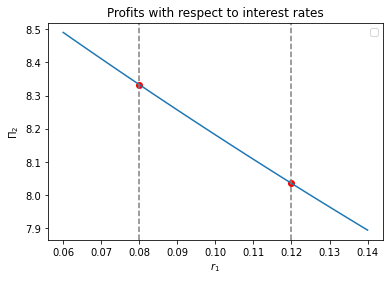
\includegraphics[width=0.7\textwidth]{media/output.png}
    \label{fig:mon_graphique}
\end{figure}
Consider the previous graph, if interest rates are $0.08$, then firms invest to reach $\Pi_2(0.08)$, but at the cost of the trade balance, meaning the interest rate will actually be $0.12$, firms will thus invest to reach $\Pi_2(0.12)$, improving the trade balance, thus interest rates will come back to $0.08$, and so on.
\newpage




\section{Interest Rate Uncertainty}
In a similar way to the previous exercises, this framework leads to the following IBC for households :
\begin{alignat}{2}
    C_1 + \frac{C_2}{1+r^*}  = Y + \frac{Y}{1+r^*} = Y\left(\frac{2+r^*}{1+r^*}\right) \equiv W(r^*) &\quad
\end{alignat}
Recall that $B_0^h = B_2^h = 0$.\newline
Let $U$ denote the lifetime utility function, $U$ writes : 
\begin{equation}
    U(C)  = \ln (C_1) + \frac{1}{2} \left[ \ln \Big((1-\sigma)(W(-\sigma)-C_1)\Big) + \ln \Big((1+\sigma)(W(\sigma)-C_1)\Big)\right]
\end{equation}
The first order condition of this maximization problem yields :
\begin{alignat}{2}
    \frac{1}{C_1}  &= \frac{1}{2}\left[ \frac{1}{W(-\sigma)-C_1} + \frac{1}{W(\sigma)- C_1}  \right]   &\quad\
    \label{46}
\end{alignat}
We will use later that $C_1 = Y$ is an immediate solution to \eqref{46} for any $\sigma \in [0, 1[$. We denote this property $(*)$. 
\subsection{}
Assuming $\sigma = 0$, \eqref{46} becomes :
\begin{alignat}{2}
    \frac{1}{C_1}  &= \frac{1}{2Y- C_1}   &\quad\
    \label{47}
\end{alignat}
And then, $C_1 = C_2 = Y$, which is the expected result as $r^*$ is known and equal to zero. In this framework, $CA_1 = TB_1 + r^* B_0 = TB_1 = Y - C_1 = 0$.
\subsection{}
In this question, we assume that $\sigma > 0$.\newline 
The budget constraint for the first period is : 
$$C_1 + B_1 = Y$$
For the second period with $r^* = \sigma$ and $r^* = -\sigma$: 
$$C_2^H = (1+\sigma) B_1 + Y = (2+\sigma)Y - (1+\sigma)C_1$$
$$C_2^L = (1-\sigma) B_1 + Y = (2-\sigma)Y - (1-\sigma)C_1$$
\subsection{}
One can now rewrite \eqref{46} as : 
\begin{alignat}{2}
    \frac{1}{C_1}  &= \frac{1}{2}\left[ \frac{1+\sigma}{C_2^H} + \frac{1-\sigma}{C_2^L}  \right]   &\quad\
\end{alignat}
\subsection{}
According to $(*)$, $C_1 = Y$ is a solution to \eqref{46}. \newline
In addition, let $f$ and $g$ denote :
\begin{align}
    f :
    \begin{cases}
        \mathbb{R_+^*} &\to \mathbb{R_+^*} \\
        x &\mapsto \frac{1}{x}
    \end{cases} &&
    g :
    \begin{cases}
        [0, W(-\sigma)[ &\to \mathbb{R_+^*} \\
        x &\mapsto \frac{1}{2}\left[ \frac{1}{W(-\sigma)-x} + \frac{1}{W(\sigma)- x}  \right]
    \end{cases}
\end{align}
One can show that :
\begin{itemize}
    \item $f$ and $g$ are well defined because $W(-\sigma) \leq W(\sigma)$
    \item $f$ is strictly decreasing
    \item $g$ is strictly increasing
\end{itemize}
Thus, the solution $C_1 = Y$ is unique.\newline
The solution is identical to the situation $\sigma = 0$. One explanation could be that the uncertainty is centered around 0. Thus the good outcome ($r^*=\sigma$) would push household to smooth consumption while the other one ($r^*=-\sigma$) would push them to consume more in the first period. Even though consumers are risk averse (concave utility) the wealth effect of a change in interest rates balances risk aversion out.
\subsection{}
Let $U$ denote the new lifetime utiliy function, $U$ writes :
\begin{equation}
    U(C) = \frac{C_1^{1-\gamma}}{1-\gamma} + \frac{1}{2}\left[  \frac{\Big((1-\sigma)(W(-\sigma)-C_1)\Big)^{1-\gamma}}{1-\gamma} + \frac{\Big((1+\sigma)(W(\sigma)-C_1)\Big)^{1-\gamma}}{1-\gamma}\right] 
\end{equation}
The first order condition yields :
\begin{equation}
    \frac{1}{C_1^{\gamma}} = \frac{1}{2} \left[ \frac{(1-\sigma)^{1-\gamma}}{\Big(W(-\sigma) - C_1)\Big)^{-\gamma}} + \frac{(1+\sigma)^{1-\gamma}}{\Big(W(\sigma) - C_1)\Big)^{-\gamma}}  \right]
\end{equation}
To which $C_1 = Y$ is an immediate solution.
Adapting the reasoning in 3.4, one can show that this solution is unique and that the results to questions 3.1 to 3.4 are identical to a log utility framework.
\subsection{}
In this question, we assume that $Y_1 = 0$ and $Y_2 = Y > 0$ so that the IBC becomes :
\begin{equation}
    C_1 + \frac{C_2}{1 + r^*} = \frac{Y}{1 + r^*} \equiv W(r^*)
\end{equation}
The FOC yields :
\begin{alignat}{2}
    \frac{1}{C_1}  &= \frac{1}{2}\left[ \frac{1}{W(-\sigma)-C_1} + \frac{1}{W(\sigma)- C_1}  \right]   &\quad\
\end{alignat}
Assuming $\sigma = 0$ implies that $\displaystyle C_1 = C_2 = \frac{Y}{2} > 0$.\newline
We also have $\displaystyle CA_1 = TB_1 = Y_1 - C_1 = - \frac{Y}{2} < 0$.\newline
The agent borrows in the first period to smooth consumption.
\subsection{}
In this question, we assume that $Y_1 = Y > 0$ and $Y_2 = 0$ so that the IBC becomes :
\begin{equation}
    C_1 + \frac{C_2}{1 + r^*} = Y \equiv W
\end{equation}
The intertemporal wealth thus does not depend on interest rate $r^*$.
The solution to solve then becomes :
\begin{alignat}{2}
    \frac{1}{C_1}  &= \frac{1}{Y-C_1}   &\quad\
\end{alignat}
Implying that : $C_1 = \displaystyle \frac{Y}{2}$ and $C_2 = (1 + r^*) \displaystyle \frac{Y}{2}$.\newline
Thus the households purchases $B_1 = \displaystyle \frac{Y}{2}$ of bonds in the first period whatever the value of $\sigma$.\newline
In this framework, $CA_1 = TB_1 = Y - C_1 = \displaystyle \frac{Y}{2} > 0$, again, whatever the value of $\sigma$.



\newpage
\section{Distortionary Taxation}
\subsection{}
\subsubsection*{Household}
The IBC for households writes :
\begin{equation}
    (1 + \tau_1)C_1 + \frac{(1+\tau_2)C_2}{1+r^*} = Y_1 - T^L + \frac{Y_2}{1+r^*} \equiv W^h
\end{equation}
\subsubsection*{Government}
The IBC for the government writes :
\begin{equation}
    G_1 + \frac{G_2}{1+r^*} = \tau_1 C_1 + T^L + \frac{\tau_2 C_2}{1+r^*}
\end{equation}
\subsubsection*{Economy}
The constraint for the whole economy writes :
\begin{equation}
    C_1 + \frac{C_2}{1+r^*} = Y_1 - G_1 + \frac{Y_2 - G_2}{1+r^*} \equiv W
\end{equation}
\subsection{}
The FOC for the household maximization problem yields :
\begin{equation}
    \frac{1}{C_1} = \frac{(1 + \tau_1)\beta}{W - (1 + \tau_1)C_1}
\end{equation}
Which implies :
\begin{alignat}{2}
    C_1 &= \frac{1}{(1+\beta)(1+\tau_1)}W^h &\quad\\
    C_2 &= \frac{\beta(1+r^*)}{(1+\beta)(1+\tau_2)}W^h &\quad 
\end{alignat}
\subsection{}
Inserting the expressions for $C_1$ and $C_2$ in the intertemporal constraint for the whole economy :
\begin{equation}
    \alpha W^h = W
\end{equation}
With $\alpha$ denoting :
\begin{equation}
    \alpha = \frac{1}{(1+\beta)(1+\tau_1)} + \frac{\beta}{(1+\beta)(1+\tau_2)}
\end{equation}
Solving for $T^L$ :
\begin{equation}
    T^L = Y_1 + \frac{Y_2}{(1+r^*)} - \frac{W}{\alpha}
\end{equation}
Using a python script to make the computation, I find :
\begin{align*}
    T^L = 0.76  && \quad
    C_1 = 8.0 &&\quad
    C_2 = 7.27 &\quad 
\end{align*}
Which implies :
\begin{align*}
    TB_1 = Y_1 - C_1 - G_1 = 0 
\end{align*}
\subsection{}
One can first find the value of $\tau_2$ which verifies (64) under $T^L = 0.76$ and $\tau_1 = 0.1$.
Solving (64) for $\alpha$ and then solving for $\tau_2$ (an argument of $\alpha$ viewed as a function) :

$$\frac{1}{1+\tau_2} = \frac{W(1+\beta)}{\beta \Big( Y_1 + \displaystyle \frac{Y_2}{1+r^*} \Big) - T^L} - \frac{1}{\beta(1+\tau_1)}$$

Using a script, I find $\tau_2 = 0.32$
Which allow me to rerun my previous code to find : $C_1 = 8.69$, $C_2 = 6.58$ and $TB_1 = -0.69$\newline
In the initial situation utiliy was $U_i = 3.88$ while the final utility is $U_f = 3.87$. Thus the new tax reform is not increasing utility for households.





\end{document}


